\begin{figure}

\centering





\tikzset{every picture/.style={line width=0.75pt}} %set default line width to 0.75pt        

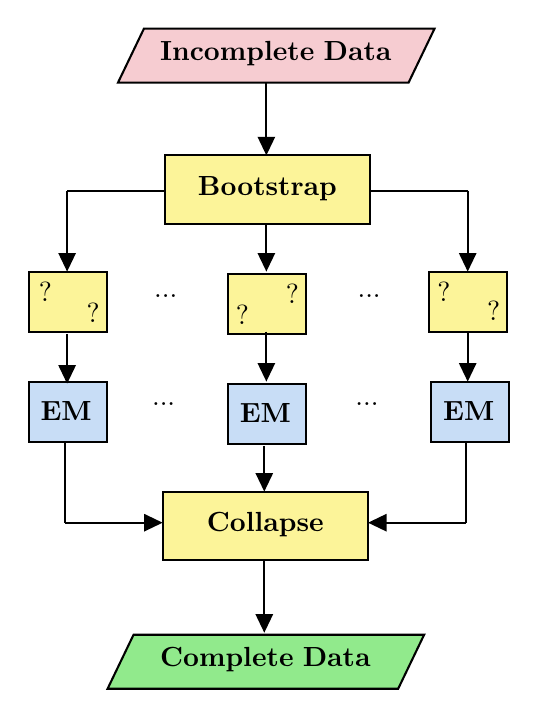
\begin{tikzpicture}[x=0.75pt,y=0.75pt,yscale=-1,xscale=1]
%uncomment if require: \path (0,652); %set diagram left start at 0, and has height of 652

\draw  [fill={rgb, 255:red, 208; green, 2; blue, 27 }  ,fill opacity=0.2 ] (244.5,3) -- (384.5,3) -- (372,29) -- (232,29) -- cycle ;
\draw    (303.5,29) -- (303.5,62) ;
\draw [shift={(303.5,64)}, rotate = 270] [fill={rgb, 255:red, 0; green, 0; blue, 0 }  ][line width=0.75]  [draw opacity=0] (8.93,-4.29) -- (0,0) -- (8.93,4.29) -- cycle    ;

\draw  [fill={rgb, 255:red, 248; green, 231; blue, 28 }  ,fill opacity=0.45 ] (254.5,64) -- (353.5,64) -- (353.5,97) -- (254.5,97) -- cycle ;
\draw    (207.5,81) -- (254.5,81) ;


\draw    (353.5,81) -- (400.5,81) ;


\draw    (207.5,81) -- (207.5,118) ;
\draw [shift={(207.5,120)}, rotate = 270] [fill={rgb, 255:red, 0; green, 0; blue, 0 }  ][line width=0.75]  [draw opacity=0] (8.93,-4.29) -- (0,0) -- (8.93,4.29) -- cycle    ;

\draw    (400.5,81) -- (400.5,118) ;
\draw [shift={(400.5,120)}, rotate = 270] [fill={rgb, 255:red, 0; green, 0; blue, 0 }  ][line width=0.75]  [draw opacity=0] (8.93,-4.29) -- (0,0) -- (8.93,4.29) -- cycle    ;

\draw    (303.5,97) -- (303.5,118) ;
\draw [shift={(303.5,120)}, rotate = 270] [fill={rgb, 255:red, 0; green, 0; blue, 0 }  ][line width=0.75]  [draw opacity=0] (8.93,-4.29) -- (0,0) -- (8.93,4.29) -- cycle    ;

\draw  [fill={rgb, 255:red, 248; green, 231; blue, 28 }  ,fill opacity=0.45 ]  (189, 120) rectangle (226.5, 149)   ;
\draw  [fill={rgb, 255:red, 248; green, 231; blue, 28 }  ,fill opacity=0.45 ]  (285, 121) rectangle (322.5, 150)   ;
\draw  [fill={rgb, 255:red, 248; green, 231; blue, 28 }  ,fill opacity=0.45 ]  (382, 120) rectangle (419.5, 149)   ;
\draw    (207.5,150) -- (207.5,172) ;
\draw [shift={(207.5,174)}, rotate = 270] [fill={rgb, 255:red, 0; green, 0; blue, 0 }  ][line width=0.75]  [draw opacity=0] (8.93,-4.29) -- (0,0) -- (8.93,4.29) -- cycle    ;

\draw    (303.5,149) -- (303.5,171) ;
\draw [shift={(303.5,173)}, rotate = 270] [fill={rgb, 255:red, 0; green, 0; blue, 0 }  ][line width=0.75]  [draw opacity=0] (8.93,-4.29) -- (0,0) -- (8.93,4.29) -- cycle    ;

\draw    (400.5,149) -- (400.5,171) ;
\draw [shift={(400.5,173)}, rotate = 270] [fill={rgb, 255:red, 0; green, 0; blue, 0 }  ][line width=0.75]  [draw opacity=0] (8.93,-4.29) -- (0,0) -- (8.93,4.29) -- cycle    ;

\draw  [fill={rgb, 255:red, 74; green, 144; blue, 226 }  ,fill opacity=0.3 ]  (189, 173) rectangle (226.5, 202)   ;
\draw  [fill={rgb, 255:red, 74; green, 144; blue, 226 }  ,fill opacity=0.3 ]  (285, 174) rectangle (322.5, 203)   ;
\draw  [fill={rgb, 255:red, 74; green, 144; blue, 226 }  ,fill opacity=0.3 ]  (383, 173) rectangle (420.5, 202)   ;
\draw    (206.5,202) -- (206.5,241) ;


\draw    (399.5,202) -- (399.5,241) ;


\draw    (302.5,204) -- (302.5,224) ;
\draw [shift={(302.5,226)}, rotate = 270] [fill={rgb, 255:red, 0; green, 0; blue, 0 }  ][line width=0.75]  [draw opacity=0] (8.93,-4.29) -- (0,0) -- (8.93,4.29) -- cycle    ;

\draw    (206.5,241) -- (251.5,241) ;
\draw [shift={(253.5,241)}, rotate = 180] [fill={rgb, 255:red, 0; green, 0; blue, 0 }  ][line width=0.75]  [draw opacity=0] (8.93,-4.29) -- (0,0) -- (8.93,4.29) -- cycle    ;

\draw    (354.5,241) -- (399.5,241) ;

\draw [shift={(352.5,241)}, rotate = 0] [fill={rgb, 255:red, 0; green, 0; blue, 0 }  ][line width=0.75]  [draw opacity=0] (8.93,-4.29) -- (0,0) -- (8.93,4.29) -- cycle    ;
\draw  [fill={rgb, 255:red, 248; green, 231; blue, 28 }  ,fill opacity=0.45 ] (253.5,226) -- (352.5,226) -- (352.5,259) -- (253.5,259) -- cycle ;
\draw    (302.5,259) -- (302.5,292) ;
\draw [shift={(302.5,294)}, rotate = 270] [fill={rgb, 255:red, 0; green, 0; blue, 0 }  ][line width=0.75]  [draw opacity=0] (8.93,-4.29) -- (0,0) -- (8.93,4.29) -- cycle    ;

\draw  [fill={rgb, 255:red, 139; green, 233; blue, 134 }  ,fill opacity=0.95 ] (239.5,295) -- (379.5,295) -- (367,321) -- (227,321) -- cycle ;

\draw (308,15) node   {$\mathbf{Incomplete\ Data}$};
\draw (304,80) node   {$\mathbf{Bootstrap}$};
\draw (197,130) node  [align=left] {?};
\draw (220,140) node  [align=left] {?};
\draw (292,141) node  [align=left] {?};
\draw (316,131) node  [align=left] {?};
\draw (389,130) node  [align=left] {?};
\draw (413,139) node  [align=left] {?};
\draw (207,187) node   {$\mathbf{EM}$};
\draw (303,188) node   {$\mathbf{EM}$};
\draw (401,187) node   {$\mathbf{EM}$};
\draw (303,242) node   {$\mathbf{Collapse}$};
\draw (303,307) node   {$\mathbf{Complete\ Data}$};
\draw (255,132) node   {$...$};
\draw (353,132) node   {$...$};
\draw (254,184) node   {$...$};
\draw (352,184) node   {$...$};


\end{tikzpicture}

\caption[BEM procedure]{\textit{Bootstrapped Expectation Maximization (BEM) procedure}}
\label{fig:BEM_algo}

\end{figure}